\documentclass[a4paper, 12pt]{book}
\usepackage{graphicx}
\usepackage[french]{babel}
\usepackage[utf8]{inputenc}
\usepackage{textcomp}
\usepackage[T1]{fontenc}
\usepackage{multirow}

\usepackage[table]{xcolor}

\usepackage{listings}
\usepackage{float}
\usepackage{url}
\usepackage[french]{algorithm}
\usepackage{style/myalgorithm}
\usepackage{amsmath,amsfonts,amssymb, commath}
\usepackage{biblatex}
\addbibresource{memoire}
\newcommand{\fBm}{\emph{fBm}~}
\newcommand{\etal}{\emph{et al.}~}
\newcommand{\glAd}{\emph{GL4D}~}
\newcommand{\apiopengl}{API OpenGL\textsuperscript{\textregistered}~}
\newcommand{\opengl}{OpenGL\textsuperscript{\textregistered}~}
\newcommand{\opengles}{OpenGL\textsuperscript{\textregistered}ES~}
\newcommand{\clang}{langage \texttt{C}}
\newcommand{\codesource}{\textsc{Code source}~}
\floatstyle{ruled}
\newfloat{programslist}{htbp}{locs}
\newcommand{\listofprograms}{\listof{programslist}{Liste des codes source}}
\newcounter{program}[subsection]
\renewcommand{\theprogram}{\arabic{chapter}.\arabic{program}}

\newenvironment{program}[1]{
  \if\relax\detokenize{#1}\relax
  \gdef\mycaption{\relax}
  \else
  \gdef\mycaption{#1}
  \fi
  \refstepcounter{program}
  \addcontentsline{locs}{section}{#1}
  \footnotesize
}{
  \begin{description}
    \item[\codesource \theprogram]--~\mycaption
  \end{description}
}

\begin{document}
\begin{titlepage}
  \begin{center}
    %\begin{tabular*}{\textwidth}{l@{\extracolsep{\fill}}r}
      
\includegraphics[height=2.5cm, width=6cm]{images/paris8Logo.png}
    %\end{tabular*}
    \small 
    \rule{\textwidth}{.5pt}~\\
    \large 
    \textsc{Université Paris 8 - Vincennes à Saint-Denis}\vspace{0.5cm}\\
    \textbf{Master 1 Informatique}\vspace{3.0cm}\\
    \Large
    \textbf{Mémoire projet tuteuré}\\
    \textbf{Qualification de caméras RGB-D}\vspace{1.5cm}\\
    
    \large
    \textbf{Yasmine BOUDJEMAÏ}\\
\textbf{Mélanie DE JESUS CORREIA}\vspace{1.5cm}\\
    Date de soutenance : le 10/01/2020\\
  \end{center}\vspace{3.5cm}~\\
  \begin{tabular}{ll}
    \hspace{-0.45cm}Organisme~:~&~Université Paris 8 Vincennes-Saint-Denis\\
    \hspace{-0.45cm}Tuteur~:~&~Farès  \textsc{BELHADJ}\\
  \end{tabular}
\end{titlepage}
\frontmatter



\chapter*{Dédicaces}
\markboth{\sc Dédicaces}{}


\chapter*{Remerciements}
\markboth{\sc Remerciements}{}

\chapter*{Résumé}
\markboth{\sc Résumé}{}


%% Table des matières
\tableofcontents
%% La liste des figure est optionnelle (si votre rapport manque de
%% contenu ajouter ce type de pages sera perçu négativement)
\listoffigures
%% La liste des programmes est optionnelle (si votre rapport manque de
%% contenu ajouter ce type de pages sera perçu négativement)
%\listofprogram
\mainmatter
\chapter*{Introduction}
\markboth{\sc Introduction}{}
\addcontentsline{toc}{chapter}{Introduction}
La caméra RGB-D dans ses débuts, notamment la Kinect, a beaucoup
servi le monde du jeux-vidéo. Cependant, depuis un certain nombre d'années, elle contribue activement et fondamentalement dans le développement
de multiples applications dans diverses disciplines telles que la médecine, la
robotique et plus généralement l'aide à la personne.
\par Ce projet tuteuré a pour objet la conception d'outils pour la qualification de caméras RGB-D. Il vise à comparer différentes caméras afin de sélectionner la meilleure en
fonction du besoin ciblé.
\par L'application résultante de ce projet devra être en mesure de détecter la colonne vertébrale de la personne posant de dos à la caméra RGB-D, principalement ceux atteints par la scoliose. Ainsi, nous nous attendons à ce qu'elle puisse modéliser la colonne en partant d'un modèle 3D et produire par la suite un rapport des mesures effectuées avec chacune des caméras. 
\par Cependant, comme dans tout projet, des contraintes s'imposent. Parmi ces dernières, nous pouvons citer:
\begin{itemize}
	\item La localisation de la colonne vertébrale. Pour cela, nous pensons utiliser le Machine Learning pour vérifier si le patient est atteint de scoliose. Si tel est le cas, arriver à détecter les positions des contours de la colonne vertébrale.
	\item Parvenir à manipuler le modèle 3D afin qu'il corresponde à la colonne vertébrale du patient.
\end{itemize}

\chapter{État de l'art}

Dans ce chapitre, nous allons définir ce qu'est une caméra RGB-D, nous énumérons certains des différents modèles existants, nous abordons brièvement les différentes techniques utilisées pour la récupération de la profondeur par une caméra. Enfin, nous discutons les différences recensées sur la \texttt{kinect V2} et \texttt{V3}.

\section{Description d'une caméra RGB-D}

La caméra RGB-D, aussi appelée capteur RGB-D, est une caméra fournissant en même temps une image couleur et une carte de profondeur caractérisant la distance des objets vus dans l'image. Cela est rendu possible grâce à un capteur RGB et un capteur de profondeur (D pour Depth). C'est principalement ces captures qui vont nous intéresser tout au lond des qualifications.


\section{Modèles existants}
Il existe différents modèles de caméras RGB-D. Parmi elles, nous pouvons citer la Kinect et ses différentes versions, Asus Xtion Pro Live, BlasterX Senz3D, Orbbec, Intel RealSens D415, ...
\par \texttt{La Kinect} a fait son apparition en septembre 2008. Elle a été conçue par Microsoft et était destinée pour la console de jeu XBox 360. Elle permettait aux utilisateurs d'interagir avec la console à l'aide d'une NUI \footnote{Natural User Interface (Interface Utilisateur Naturelle), se réfère à une interface utilisateur invisible.} en utilisant les mouvements gestuels et une reconnaissance vocale. Elle sera plus tard utilisée dans les domaines de la  recherche et du développement pour différents secteurs comme le domaine de la médecine, l'industrie automobile, la robotique, l'éducation,  .... 
\par \texttt{Asus Xtion Pro Live} est le modèle de référence que nous utilisons afin d'effectuer les qualifications. Elle utilise la technologie PrimeSense  \footnote{Connu principalement pour sa licence de conception matérielle et de puce employée dans le mécanisme de détection de mouvements de la Kinect XBox360. Pour plus d'informations, le lecteur peut se référer à ce lien \url{https://www.crunchbase.com/organization/primesense#section-web-traffic-by-similarweb}.} pour la détection de mouvements.
\par \texttt{BlasterX Senz3D} a fait son apparation en Septembre 2016. Conçue par Creative,  elle a été présentée comme une webcam intelligente basée sur ce qu'il y a de mieux en matière de savoir-faire et de technologie. Elle possède trois lentilles pour capturer les données visuelles: une caméra RVB, une caméra infra-rouge et un projecteur laser. Ces dernières collaborent avec la technologies Inetl RealSense pour réagir aux expressions faciales et aux gestes corporels des utilisateurs.
\par \texttt{Orbbec Astra Pro} fait partie de la série Astra. Elle offre une vision par ordinateur qui permet des dizaines de fonctions telles que la reconnaissance des visages, la reconnaissance des gestes, le suivi du corps humain, la mesure tridimensionnelle, la perception de l'environnement et la reconstruction de cartes en trois dimensions. De plus, elle offre une réactivité haut de gamme, une mesure de la profondeur, des dégradés fluides et des contours précis ainsi que la possibilité de filtrer les pixels de profondeur de faible qualité.
\par \texttt{Intel RealSense D415} a un champ de vision standard bien adapté aux applications de haute précision telle que la numérisation 3D. Elle comprend le processeur Intel RealSense Vision D4 offrant une résolution en profondeur élevée, des capacités de longue portée, une technologie d'obturation globale et un large champ de vision. Grâce à ces deux dernières, la caméra offre une perception précise de la profondeur lorsque l'objet est en mouvement ou que l'appareil est en marche. De plus, elle couvre un champ de vision plus large, minimisant ainsi les angles morts.

\section{Erreur de mesure}
L'erreur de mesure, autrefois appelée l'erreur absolue, est un processus qui permet d'évaluer l'écart entre la valeur mesurée et la valeur de référence qui est soit exacte ou connue. L'objectif de la mesure d'erreurs est de jauger à quel degré les deux valeurs sont proches. 
Dans cette section, nous citons les types ainsi que quelques sources d'erreurs, ensuite,  nous faisons un détour sur les moyens théoriques et physiques employés à cet effet.
\subsection{Types et sources d'erreurs}
Il existe deux types d'erreurs: aléatoires et systématiques. \\ Les erreurs aléatoires sont des erreurs dont les valeurs sont incohérentes et imprévisibles même en répétant les observations et en conservant les mêmes paramètres. \\Les erreurs dites systématiques, à l'inverse des erreurs aléatoires, sont des erreurs reproductibles, elles demeurent constantes tant que les paramètres restent inchangés. \\ \\
Ces erreurs peuvent résulter de différentes sources; elles peuvent être dues à des facteurs environnementaux, à la résolution de l'instrument utilisé, au calibrage de l'appareil employé ou même à des erreurs humaines. \\ \\
\subsection{Mesure d'erreurs à l'aide de matériels}
Diverses instruments de mesures de distance sont mis à porté des professionnels tels que les ingénieurs en génie civil, les architectes, les métreurs, les dessinateurs, les topographes, les menuisiers, les maçons, les agents immobiliers, les électriciens, les décorateurs, les experts. Nous nommons certains d'entre eux ci-après.
\begin{description}
	\item[Distancemètre laser Leica DISTO D8]: cet appareil est pourvu d'un localisateur numérique, d'un écran couleur haute résolution 2,4", d'un capteur d'inclinaison 360° et de lma technologie Bluetooth. Parmi ses caractéristiques techniques, on peut citer:
	\begin{itemize}
		\item Il possède une porté allant de 0.05m jusqu'à 200m.
		\item Une précision de $\pm 1mm$.
		\item Des opérations arithmétiques ainsi que des fonctions mathématiques sont intégrées à l'instrument telles que la fonction Pythagore, la fonction Trapèze ou encore la fonction triangle.
		\item Image en temps réel 
		\item Un Plug-In d'AutoCAD embarqué dans l'appareil qui permet de dessiner et de planifier avec le logiciel d'AutoCAD.
		\item Il inclut un logiciel de transfert de données pour le distancemètre  \textbf{Leica Disto Transfert}.
		\item Avec la technologie Bluetooth intégrée, l'utilisateur peut transférer les mesures effectuées vers un ordinateur portable ou un PC sans avoir recours aux câbles. Les données ainsi transférées peuvent être éditées à l'aide de logiciels tels que Word, Excel, AutoCAD ou encore d'autres.  
	\end{itemize}
\end{description}

\begin{description}
	\item[Odomètre vérifiable PCE-MW 2]: Instrument permettant de mesurer différentes zones (ie: chantiers, zones industrielles, zones sportives, ...), des câblages, des tuyauteries. Parmi ses caractéristiques, on peut mentionner:
	\begin{itemize}
		\item Pèse 2200g
		\item Mesure pouvant aller jusqu'à 99999,9 mètres.
		\item Permet d'effectuer une addition en se déplaçant vert l'avant et une soustraction en bougeant vers l'arrière.
		\item Possède une précision de $\pm 1\%$
		\item La roue est en plastique et permet de résister aux huiles.
	\end{itemize}	
\end{description}

\begin{description}
	\item[Distancemètre laser PCE-LRF 600]: Le design de cet instrument est bien conçu puisqu'il est léger et il permet de le maintenir avec une seule main. De plus, il est facile d'utilisation. De ses caractéristiques, on peut évoquer:
	\begin{itemize}
		\item Il pèse 165g.
		\item Il a une porté allant de 15m à 600m.
		\item Une précision de $\pm 1m/\pm 0.1\%$.
		\item Il possède un laser de type classe 1.
		\item Résistant aux éclaboussures d'eau
		\item Il permet une mesure des distances dans diverses situations météorologiques.
	\end{itemize}
	
\end{description}


\subsection{Mesure d'erreurs par une approche théorique}
A ce jour, on recense de multiples méthodes exploités à cet effet. Nous nous contentons de citer ci-dessous celles qui nous paraissent êtres les plus pertinentes. \\

\begin{description}
	\item[RMSE/RMSD]: Root Mean Square Error ou encore Root Mean Square Deviation que l'on pourrait traduire par; la racine carré de la moyenne des erreurs au carré. Elle demeure parmi les plus fréquentes en la matière. C'est une mesure de l'exactitude, qui permet de comparer les erreurs de prévision de différents modèles pour un ensemble de données précis et non entre des ensembles de données. Sa formule s'exprime comme suit:
	\begin{equation}
		\sqrt{\frac{1}{N}.\sum_{i = 1}^{N}(x_i - \hat{x_i})^2}
	\end{equation}	
De par la formule, on peut déduire que le résultat sera toujours positif et qu'obtenir une valeur de 0 (qui n'est généralement non atteint en pratique), témoignerait d'une exactitude parfaite. Ainsi, obtenir des valeurs avoisinant le zéro est positif pour les mesures.
	\item[MSE]: Mean Square Error que l'on pourrait traduire par; l'erreur quadratique moyenne. Sa formule est comme suit:
	\begin{equation}
		\frac{1}{N}.\sum_{i = 1}^{N}(x_i - \hat{x_i})^2
	\end{equation}
	
	\item[MAE]: Mean Absolute Error qui pourrait être traduit par; erreur moyenne absolue. Son équation est comme ci-dessous:
	\begin{equation}
		\frac{1}{N}.\sum_{i = 1}^{N} \abs{x_i - \hat{x_i}}
	\end{equation}	 
	\item[MAPE]: Mean Absolute Percentage Error qui pourrait être traduit par; le pourcentage de l'erreur moyenne absolue. Elle fait partie également des moyens de mesures d'erreur les plus fréquents. A noter que la valeur observée ne doit être aucunement nulle. La formule est comme ci-après:
	\begin{equation}		
		\frac{1}{N}.\sum_{i = 1}^{N} \abs{\frac{x_i - \hat{x_i}}{x_i}}
	\end{equation}
\end{description}


Avec: \\ \\
$x_i$, la valeur observée à la ième observation. \\
$\hat{x}_i$, la valeur exacte à la ième observation. \\
$N$, représente le nombre d'observations

%\section{Techniques existantes de capture de mouvements} 
\section[Technologies utilisées pour la depth]{Technologies utilisées pour la depth d'une caméra RGB-D} 
Des méthodes employées pour la récupération de la depth, on peut en citer deux principales.
\subsection{Infrarouge}
Le projecteur infrarouge de certaines caméras le possédant qu'on peut voir sur la figure \ref{fig-Asus} projette un spectre infrarouge sur la scène captée. Le motif produit sur cette dernière sera capté par la caméra infrarouge et sera par la suite comparé à la base de données de motifs de référence stockés au préalable dans la caméra. Ces derniers seront indispensables pour la mesure de la profondeur de chaque pixel. 

\begin{figure}[htbp]
  %\centering
  \hspace{-0.75cm}
 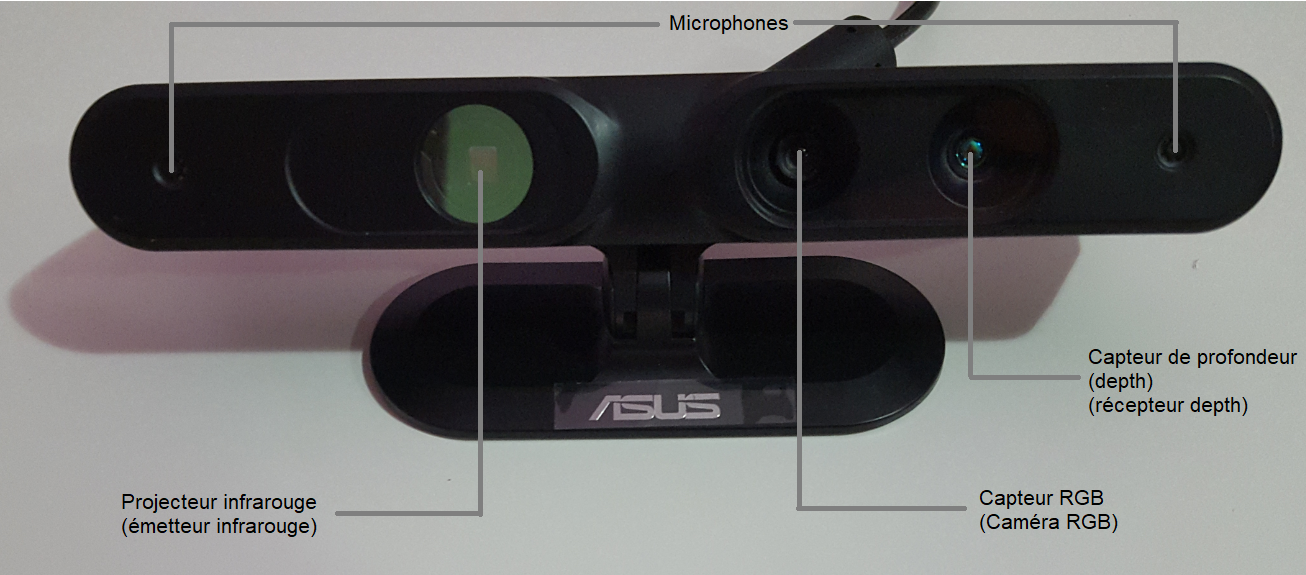
\includegraphics[scale=0.50]{images/Asus.png} \hspace{2cm}
  \caption{Composants caméra RGB-D (Ici Asus Xtion Pro Live).\label{fig-Asus}}
\end{figure}

Par la suite, les valeurs obtenues seront corrélées à un capteur RGB qu'on peut apercevoir sur la figure. Ces données pourront être représentées par un nuage de points \footnote{Est une représentation des points de coordonnées tridimensionnelles dont chacun peut avoir des attributs qui lui ont sont propres.}.


	\par Toutefois, ce type de caméras possède certaines restrictions. Parmi ces dernières, on peut citer:
	\begin{itemize}
		\item {Distances de mesure limitées.}	
		\item {Problèmes de calculs des informations de profondeur à l'encontre de surfaces brillantes, très mates, transparentes, réfléchissantes ou encore envers des objets absorbants.} 
		\item {Interférence des motifs (patterns) infrarouges si présence de plusieurs caméras RGB-D de même type. En effet, chaque capteur visualisera ses propres motifs ainsi que ceux des autres caméras présentes et ne saura distinguer les siens des autres qui se chevauchent.  De cela découle une perte considérable d'informations de profondeur comme nous pouvons l'observer sur la figure \ref{fig-interference}. 

\begin{figure}[htbp]
  %\centering
  \hspace{0.75cm}
 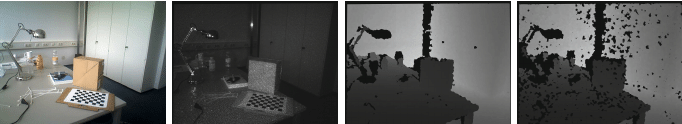
\includegraphics[scale=0.5]{images/interference.png}
  \caption{(De gauche à droite) image renvoyée par la caméra RGB, image IR, depth map (une seule caméra), depth map (deux caméras). (figure tirée de l'article de \emph{F.Alhwarin, A.Ferrein} et \emph{I.Scholl} ayant comme titre \emph{IR Stereo Kinect: Improving Depth Images by Combining StructuredLight with IR Stereo}).\label{fig-interference}}
\end{figure}

Cependant, des travaux de recherches ont été conduits afin d'y remédier. Parmi eux, on peut citer le travail réalisé par l'équipe de \emph{Rafibakhsh} ( \cite{RAFIBAKHSH15}) qui recommande de laisser un angle de 35\textdegree{} entre deux caméras suspendues à la même hauteur en considérant les scènes captées dans de bonnes conditions et une interférence très faible. \emph{Maimone} et \emph{Fuchs} \cite{MaimoneFuchs15} proposent un algorithme de remplissage et de lissage en modifiant le filtre médian aux zones trouées à l'exception des bords. Quant à \emph{F. Kenton Musgrave, Craig E.} et \emph{Robert S. Mace} \cite{KentonCraigMace12}, ils appliquent une certaine quantité minime de mouvements (en utilisant des composants matériels supplémentaires) à certains capteurs de sorte que chacun puisse voir son propre motif infrarouge de façon nette et une version floue des motifs de ses voisins. }
	\end{itemize}
\subsection{Stéréo-vision}
Une caméra stéréoscopique est un appareil qui contient deux voire plus de capteurs d'images. Ceci nous rappelle la vision binoculaire humaine. En effet, ce mécanisme permet au système nerveux central de percevoir simultanément les images issus de chaque œil envoyées sous forme de signaux. Ainsi, il sera en mesure de se servir de ces différences (entre les deux images)  pour permettre une vision stéréoscopique pour la perception de relief et une mesure des distances en utilisant la triangulation \footnote{Approche géométrique permettant une mesure des distances. Le lecteur peut consulter cette page web pour de plus amples informations: \url{https://fr.wikipedia.org/wiki/Triangulation} .}. Le concept que nous venons d'expliquer est appelé disparité stéréoscopique \footnote{Différence dans la localisation d'un objet perçu par l'œil gauche et l'œil droit résultant de la séparation horizontale des yeux dont certaines caméras essaient de s'approprier la technique afin de récupérer la profondeur.}. 
\par La stéréo-vision sert principalement à reconstituer la scène observée sous forme de modèle 3D. 
\subsubsection{Carte de disparités}
Le principe de la disparité est une approche du mécanisme humain vu précédemment. Il consiste en la différence entre les coordonnées pixels d'un point bidimensionnel d'une image et celles de son correspondant (présent sur une autre image prise au même moment). Ainsi, en appliquant le même traitement sur tous les pixels correspondants, on obtient la carte des disparités. Une carte est dite éparse lorsqu'une disparité est associée à quelques pixels et lorsque cette dernière est associée à chaque pixel, on dit d'elle qu'elle est dense.  \\ Une formule pour calculer la profondeur en fonction de la disparité s'obtient comme suit: \\ \\
\begin{equation}
 z = \dfrac{B.f}{d}  
\end{equation} 
\\ Avec: \\ \\
$z$ représentant la profondeur. \\
$B$ \emph{Baseline} représente la distance séparant les deux capteurs. \\
$f$ La distance focale en pixels calculée comme montré ci-après en nous servant de la figure \ref{fig-focal} . \\
\begin{figure}[htbp]
  %\centering
  \hspace{-3cm}
 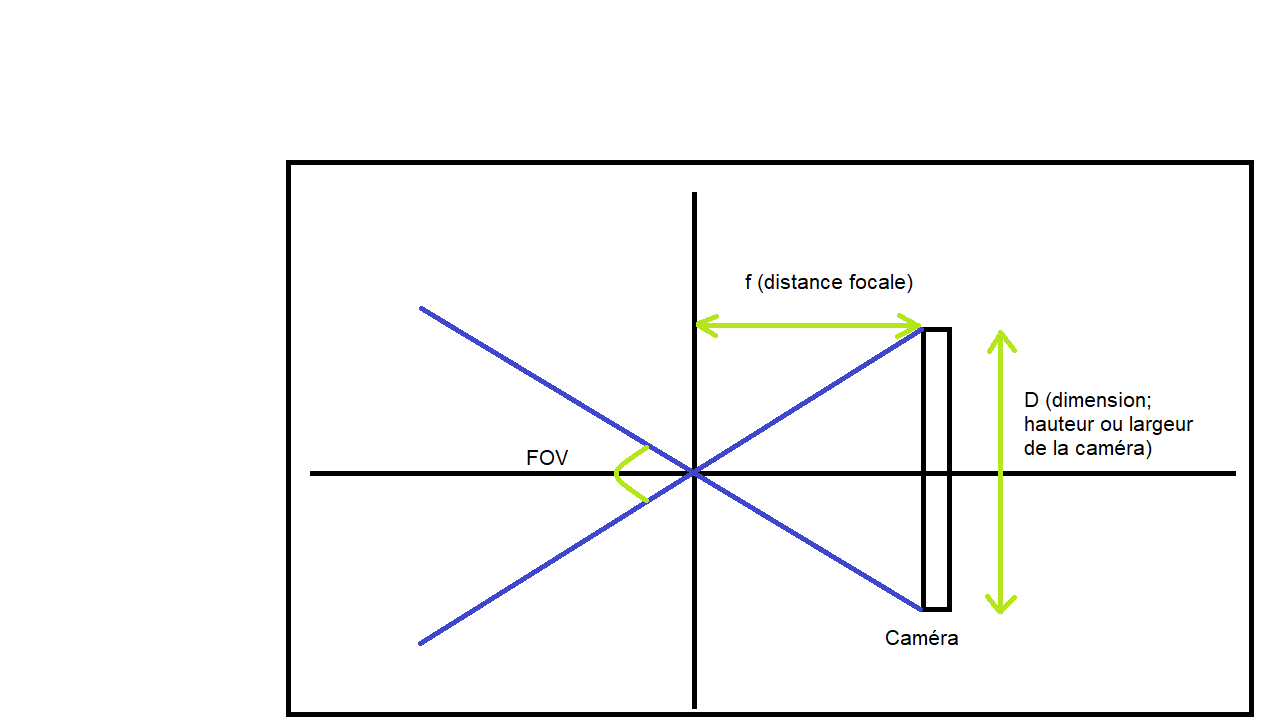
\includegraphics[scale=0.5]{images/focalLength.png} \hspace{2cm}
  \caption{Schéma illustrant la relation entre la distance focale et le champ de vision (fov).\label{fig-focal}}
\end{figure}


\begin{equation}
 \tan \left( {\dfrac{fov}{2}}\right) = \dfrac{D}{2.f}    \Leftrightarrow   f = \dfrac{D}{2. \tan \left( {\dfrac{fov}{2}}\right)}
\end{equation}
\\ Avec:\\ \\
$D$  dimension qui peut représenter soit la largeur soit la hauteur en fonction du fov de la caméra employé. \\
$fov$ (Field Of View) représente l'angle du champ de vision (soit horizontal ou vertical). \\
$f$ représente la distance focale.


\section{Kinect V2 et Kinect V3}
\subsection{Kinect V2}
\texttt{Kinect V2} se sert de la méthode TOF (ie: Time Of Flight ou autrement dit Temps De Vol) pour générer la carte de profondeur. Cette technique se base sur la différence de temps entre l'émission d'un faisceau lumineux et son retour après réflexion sur un objet. \\ La distance est calculée comme suit:\\
$ d = c.\dfrac{\Delta t}{2} $, avec $c$ la vitesse de la lumière dans l'air.\\ \par Elle permet une bien meilleure précision même dans le noir que sa version précédente (\texttt{Kinect V1)}. 

\subsection{Kinect V3}
\texttt{Kinect V3}, baptisée \texttt{Microsoft Azure Kinect V3}, tout comme la précédente version, se base aussi sur la technologie TOF. Elle comprend un capteur RGB de 12 Mp, un capteur de depth de 1Mp avec un fov réglable en large ou réduit ainsi que 7 microphones intégrés.  
 
\subsubsection{Kinect V2 Vs Kinect V3}
\texttt{Kinect V3} est beaucoup plus légère et plus petite que la \texttt{V2}. Elle possède entre autre plus de microphones que la précédente. Elle a été conçue afin d'être principalement utilisée avec Azure , le service cloud de \texttt{Microsoft}. C'est sans doute ce qui la démarque le plus de sa prédécesseure. En effet, ce service lui permet d'effectuer une partie des calculs. En outre, elle bénéficie des Cognitive Services, autrement dit de l'intelligence artificielle pourra être incluse dans les applications créées.

\chapter[Notre outil pour la qualification]{Notre outil pour la qualification de caméras RGB-D}
Dans ce passage, nous allons décrire notre outil conçu pour qualifier les caméras par rapport à notre modèle-étalon montré dans l'image ci-dessous.

\begin{figure}[htbp]
  %\centering
  \hspace{0.75cm}
 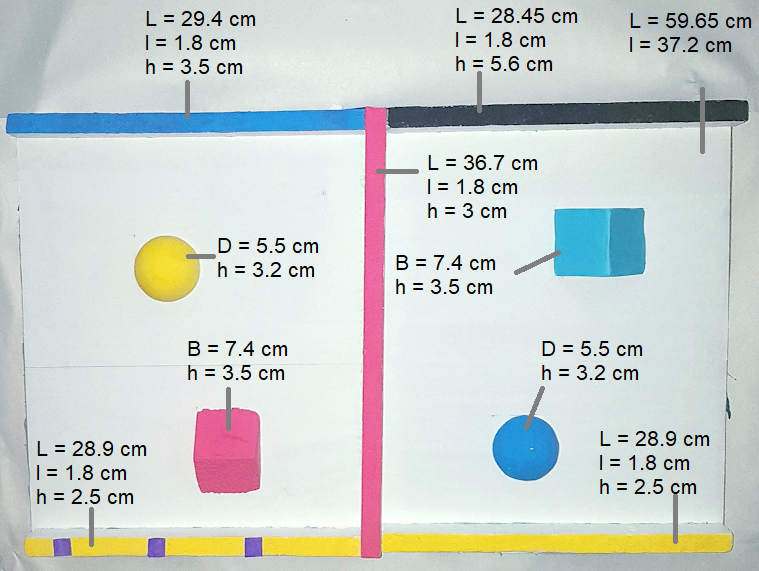
\includegraphics[scale=0.5]{images/realModel.png} \hspace{2cm}
  \caption{Modèle-étalon.\label{fig-model}}
\end{figure}

\chapter[Modèle logiciel pour la qualification]{Modèle logiciel pour la qualification de caméra RGB-D}
Dans ce passage, nous allons décrire notre outil que nous voudrions concevoir pour qualifier les caméras. Par la suite, nous montrons ce que nous avons pu commencé à faire pour débuter ce projet.


\section{Description de l'application}


\section{Application développée}
Notre application est composée d'une fenêtre qui comprend une partie affichage de la scène filmée en temps réel ainsi qu'une partie interface graphique qui nous permet de communiquer avec le programme. Nous parlerons un peu plus en détail de ces parties dans les sous-sections à venir.
\subsection{Première partie: Affichage de la scène captée }
Pour cet effet, nous sommes partis d'un programme fourni par \emph{M. Farès BELHADJ} auquel nous avons rajouté des choses pour la conception de l'outil. Il comprend l'utilisation de la bibliothèque OpenGL, GL4Dummies ainsi que la bibliothèque OpenNI2 pour établir la connexion avec la caméra RGB-D pour nous fournir par la suite la carte de couleurs et la carte de profondeurs.
\subsection{Seconde partie: Interface graphique}
Pour l'interface graphique, nous avons exploité la bibliothèque Dear ImGui disponible sur GitHub sur le lien suivant \url{https://github.com/ocornut/imgui}. C'est une bibliothèque assez facile d'utilisation une fois l'étape de l'intégration dans le contexte OpenGL effectué. Cette interface contient un certain nombre de composants. Parmi les composants principaux, nous pouvons citer une liste déroulante qui nous permet de sélectionner le modèle de caméra sur laquelle nous souhaitons réaliser les tests de mesures. Ainsi, une fois le choix de caméra effectué, le programme met automatiquement à jour tous les paramètres présents dans les champs suivants la liste en récupérant les données à partir d'un fichier que nous avons nommé \emph{infoCameras.txt}. Ainsi, ce dernier pourra être exploité pour tout rajout de nouvelles caméras et/ou modification sur les données uniquement.
Autres les composants cités ci-dessus, nous noterons la présence de deux cases à cocher comme montré dans la figure \ref{fig-gui} La première permet une détection du modèle et l'autre de passer les tests de mesures.
\begin{figure}[htbp]
  %\centering
  \hspace{3.5cm}
 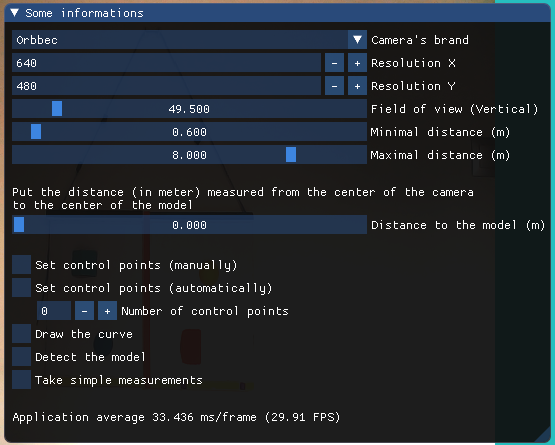
\includegraphics[scale=0.5]{images/GUI.png} \hspace{2cm}
  \caption{Interface graphique du programme.\label{fig-gui}}
\end{figure}

\section{Conception du modèle réel et du modèle virtuel}

\section{Comparaison de la depth OpenGL avec la depth de la caméra RGB-D}
Dans ce passage, nous exposons certains des résultats obtenus ainsi que les résultats attendus avec la caméra Asus.

\subsection{Résultats obtenus}

\subsection{Résultats attendus}


\chapter{Cas pratiques de qualification}

\section{Modèle 3D}
\section{La POC}
\section{Résultats et critique}


\chapter{Conclusion et Perspectives\label{chap-conclusion}}


\nocite{*}
%	\bibliographystyle{alpha}
%\bibliography{memoire}
\printbibliography
\end{document}

